\documentclass{beamer}
\usetheme{Boadilla}
\usecolortheme{sidebartab}

\usepackage{hyperref}
\usepackage{showexpl} 
\usepackage{graphicx}
\usepackage{tikz}
\usepackage{color}
\usepackage{siunitx}
\usepackage[version=3]{mhchem}
\usepackage{chemfig}
\usepackage{changes}
\usepackage[many]{tcolorbox}
\usepackage{natbib}
\bibliographystyle{unsrtnat}
\setcitestyle{square,numbers}

\beamertemplatenavigationsymbolsempty
\setbeamertemplate{footline}{}
\setbeamertemplate{bibliography item}{\insertbiblabel}

\lstloadlanguages{[LaTeX]Tex} 
\lstset{% 
     basicstyle=\ttfamily\large, 
     commentstyle=\itshape\ttfamily, 
     showspaces=false, 
     showstringspaces=false, 
     breaklines=true, 
     breakautoindent=false, 
     captionpos=t,
     explpreset={numbers=none},
     pos=b
} 

\newtcolorbox{titlebox}[1][]{
	width=1.2\textwidth,
	boxrule=0pt,
	leftrule=0pt,
	rightrule=0pt,
	toprule=0pt,
	bottomrule=0pt,
	arc=0pt,
	colback=yellow!20,
	opacityback=0.7,
	enhanced jigsaw
}

\title{Research Data and Data Management Planning}
\author{Markus Stocker}
\date{September 12, 2017}

\begin{document}

\maketitle

\begin{frame}
  \frametitle{Outline}
  
  \begin{itemize}
  \item What are research data
  \item Research data lifecycle
  \item Data types, formats, models and standards
  \item Metadata
  \item Data management, plans and planning tools
  \end{itemize}
\end{frame}

% Joan Miro (1968). Landscape. Acrylic on canvas
% Essentially a white canvas with a colored dot
% It makes for a good example for what a datum is, at least for philosophers
{
	\usebackgroundtemplate{ %
		\begin{tikzpicture}[remember picture, overlay]%
		\node at (current page.center) {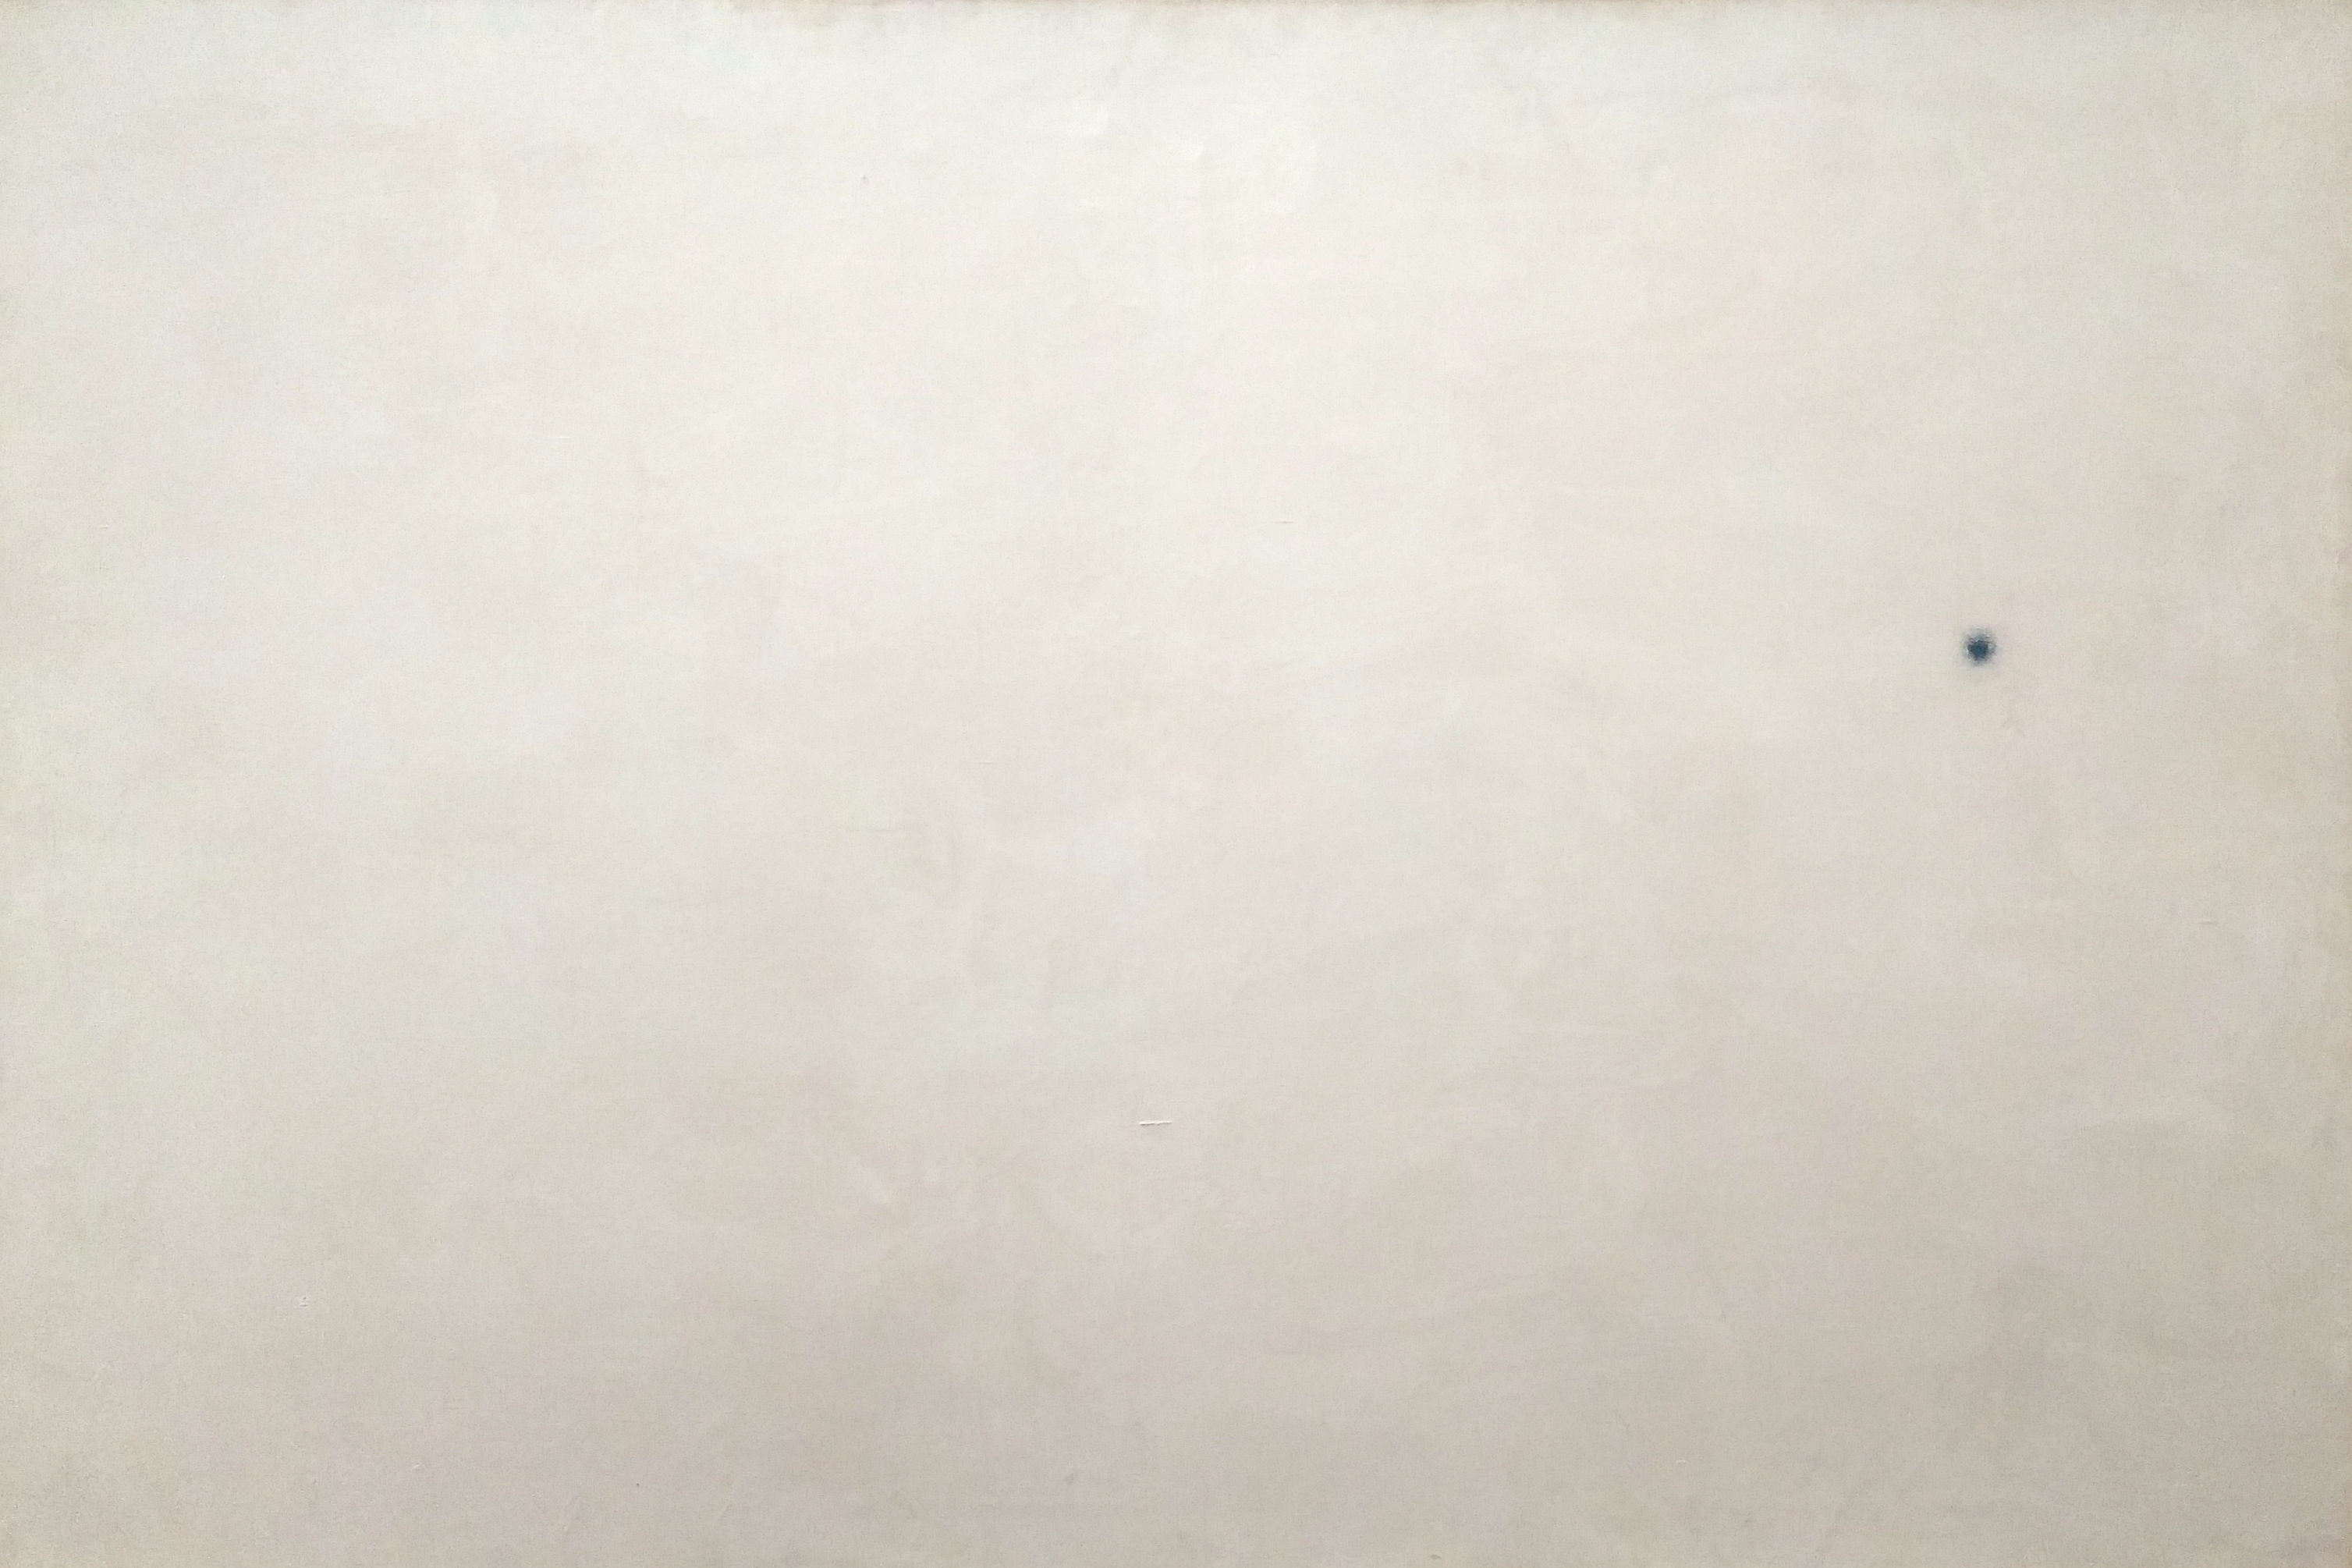
\includegraphics[height=\paperheight]{graphics/joan-miro-landscape-1968.jpg}};%
		\end{tikzpicture}%
	}%
	\setbeamertemplate{navigation symbols}{}
	\begin{frame}[plain]
	\end{frame}
}

% Datum is ultimately reducible to a lack of uniformity (between signals, symbols, ...)
% That's the reason why lights used to signal emergency flash
% Data depend on the occurrence of differences
% Defined as x being distinct from y
% Where x, y are uninterpreted (typed) variables
% Variable is a symbol that acts as a placeholder for an unknown (or changeable) referent
% Referent: the thing in the world that the symbol denotes (or stands) for
{
	\usebackgroundtemplate{ %
		\begin{tikzpicture}[remember picture, overlay]%
		\node at (current page.center) {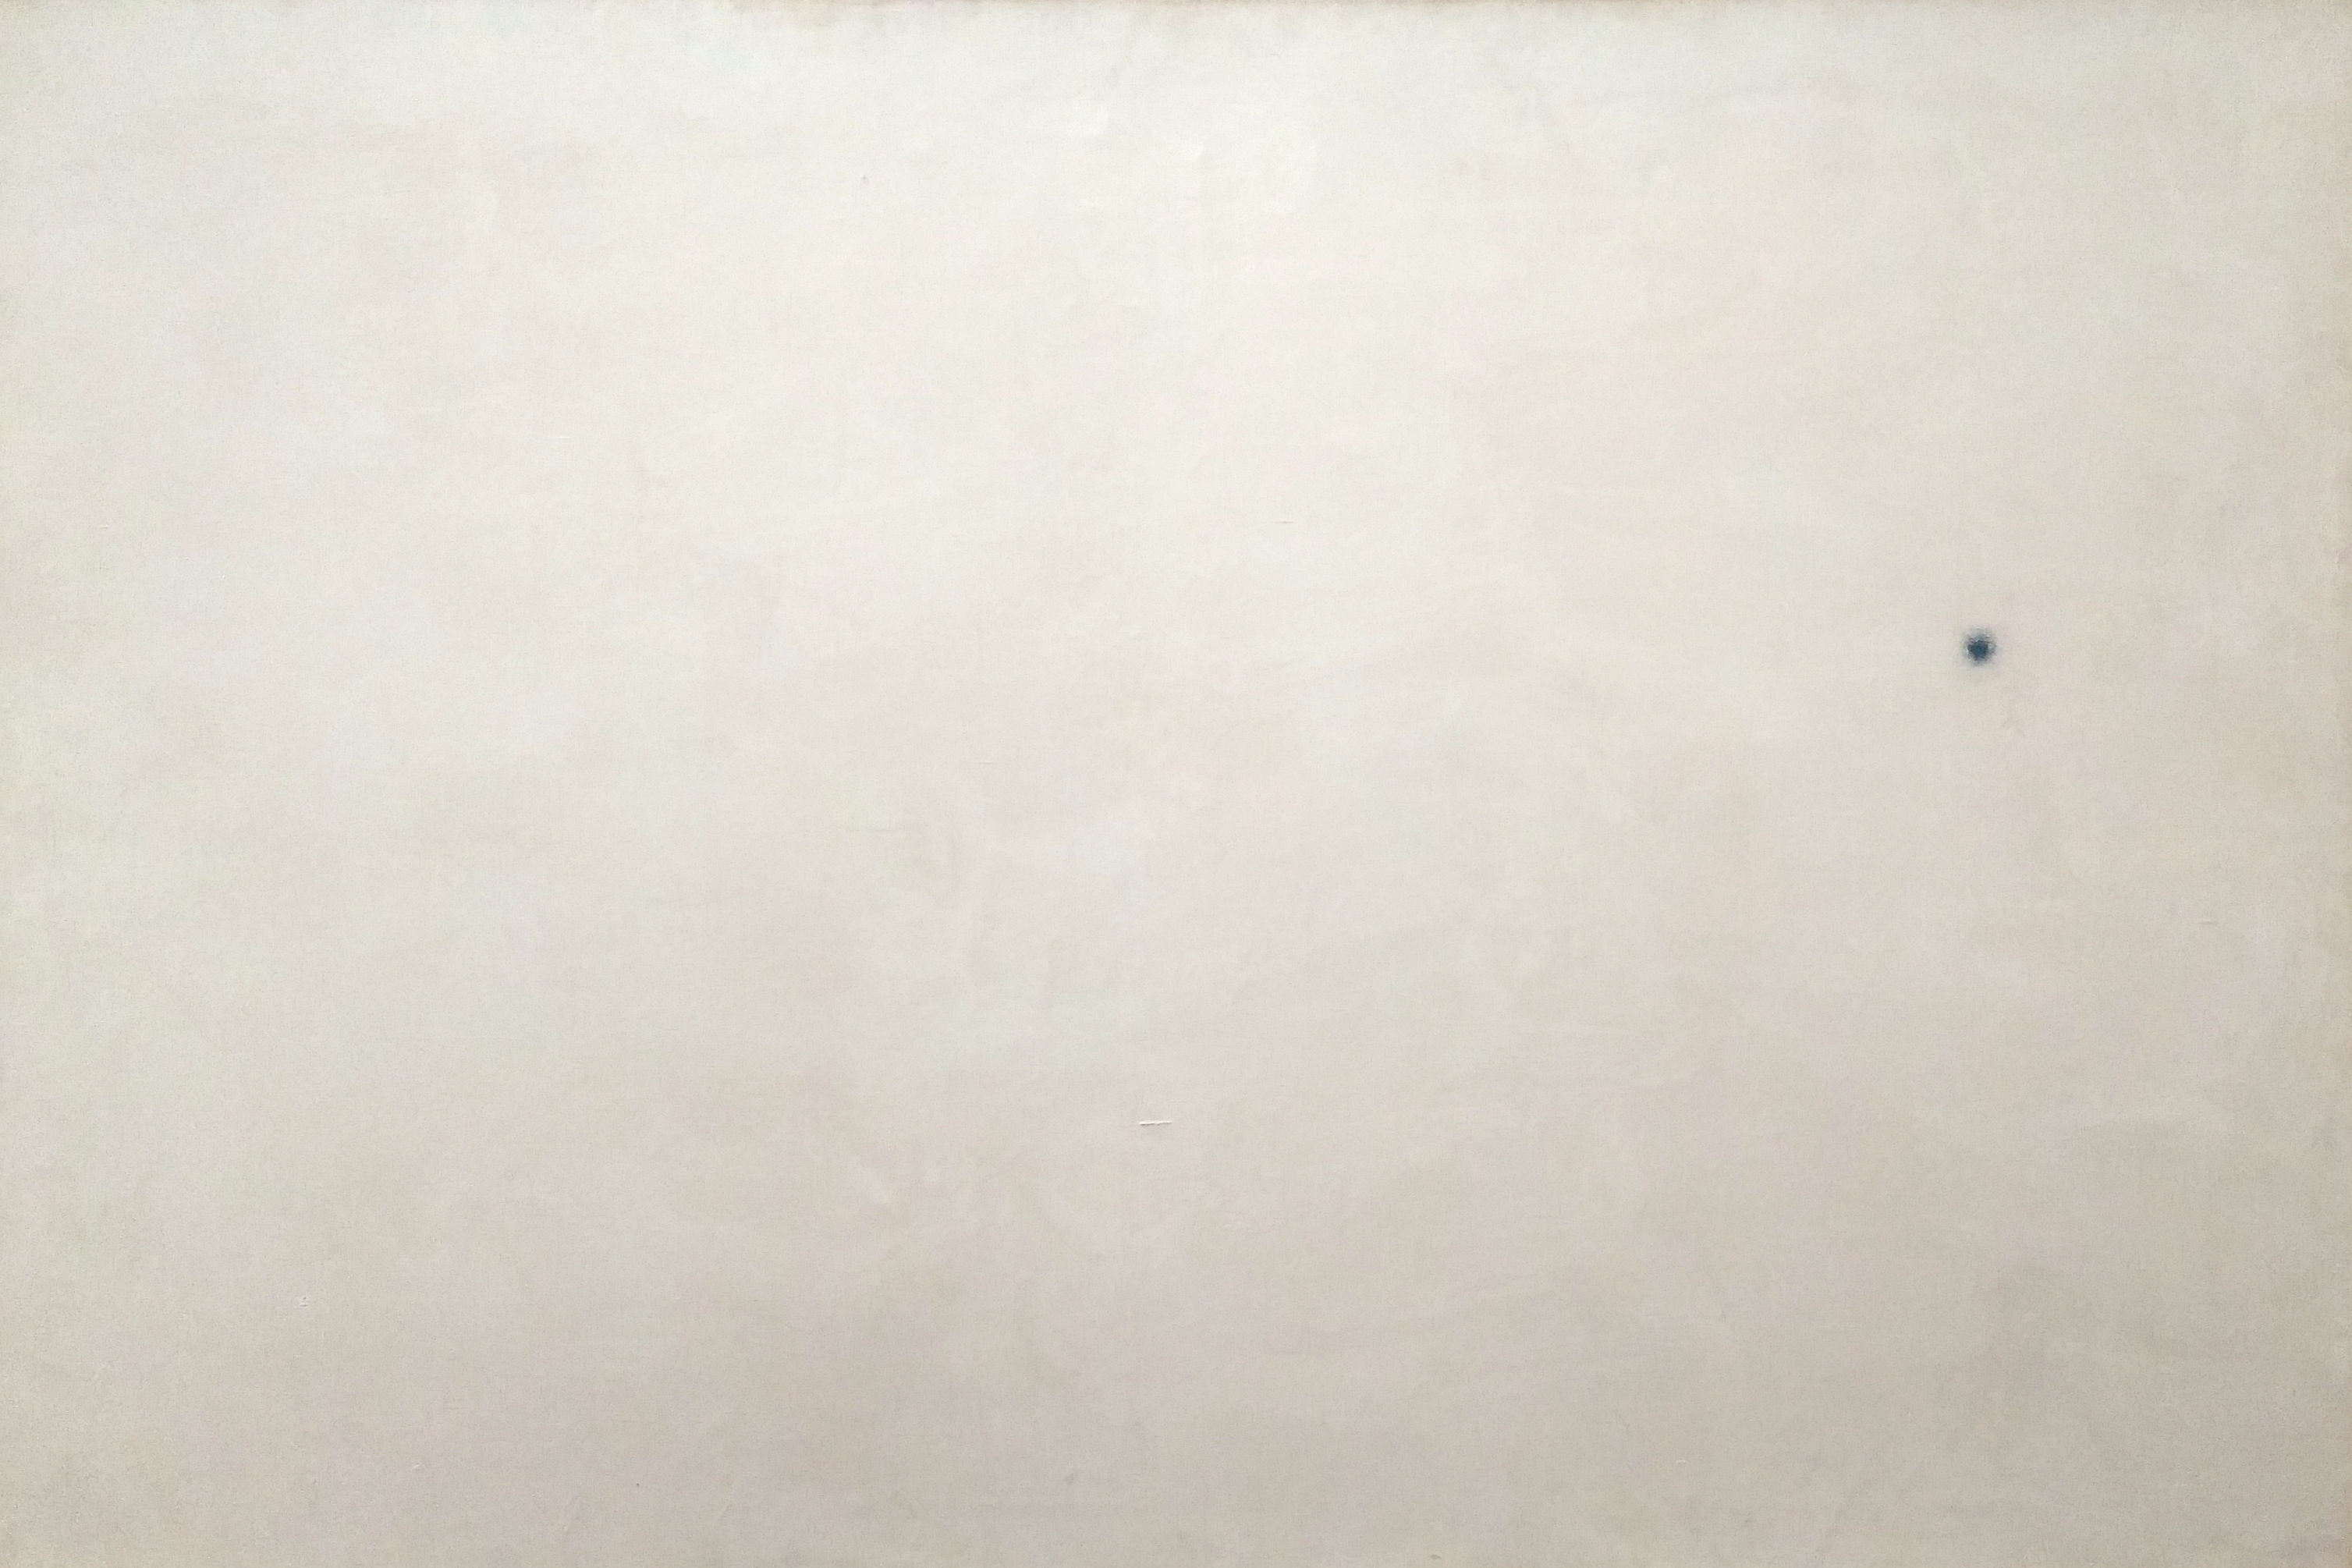
\includegraphics[height=\paperheight]{graphics/joan-miro-landscape-1968.jpg}};%
		\end{tikzpicture}%
	}%
	\setbeamertemplate{navigation symbols}{}
	\begin{frame}[plain]
	\vspace{6cm}
			\begin{tikzpicture}
				\hspace{-0.55cm}
				\node {
					\begin{titlebox}
						\large Datum is ultimately reducible to a lack of uniformity \cite{floridi11philosophy}
					\end{titlebox}
				};
			\end{tikzpicture}
	\end{frame}
}

\begin{frame}
  \frametitle{Define data}
  
  \begin{itemize}
  \item Entities, physical or digital, used as evidence of phenomena \cite{borgman15big}
  \item A reinterpretable representation of information \cite{ccsds12oais}
  \item Items of recorded information
  \item There is no consensus definition
  \item Even institutions that curate data may not define what they curate
  \end{itemize}
\end{frame}

\begin{frame}
  \frametitle{Data examples}
  
  \begin{itemize}
  \item Not just spreadsheets of numbers, also
  \item Sequences of bits
  \item Characters on a page
  \item Recording of sounds
  \item Physical and biological specimens
  \item Images
  \item Software
  \end{itemize}
\end{frame}

\begin{frame}
  \frametitle{Define research data}
  
  \begin{itemize}
  \item Unsurprisingly, there is no consensus on the definition
  \item Factual material [...] necessary to validate research findings \cite{epsrc17researchdata}
  \item Everything needed to reproduce a given scientific output \cite{surkis15researchdata}
  \item ...
  \end{itemize}
\end{frame}

\begin{frame}
  \frametitle{Research data examples}
  
  \begin{itemize}
  \item In addition to the obvious, e.g. data files
  \item Notebooks, e.g. laboratory, field, diaries, ...
  \item Questionnaires, audio and video tapes
  \item Models and scripts
  \item Workflows and protocols
  \end{itemize}
\end{frame}

% Creating data: design research; plan data management (formats, storage etc); plan consent for sharing; locate existing data; collect data (experiment, observe, measure, simulate); capture and create metadata
% Processing data: enter data, digitise, transcribe, translate; check, validate, clean data; anonymise data where necessary; describe data; manage and store data
% Analysing data: interpret data; derive data; produce research outputs; author publications; prepare data for preservation
% Preserving data: migrate data to best format; migrate data to suitable medium; back-up and store data; create metadata and documentation; archive data
% Giving access to data: distribute data; share data; control access; establish copyright; promote data
% Re-using data: follow-up research; new research; undertake research reviews; scrutinise findings; teach and learn
\begin{frame}
  \frametitle{Research data lifecycle}
  
  \begin{center}
  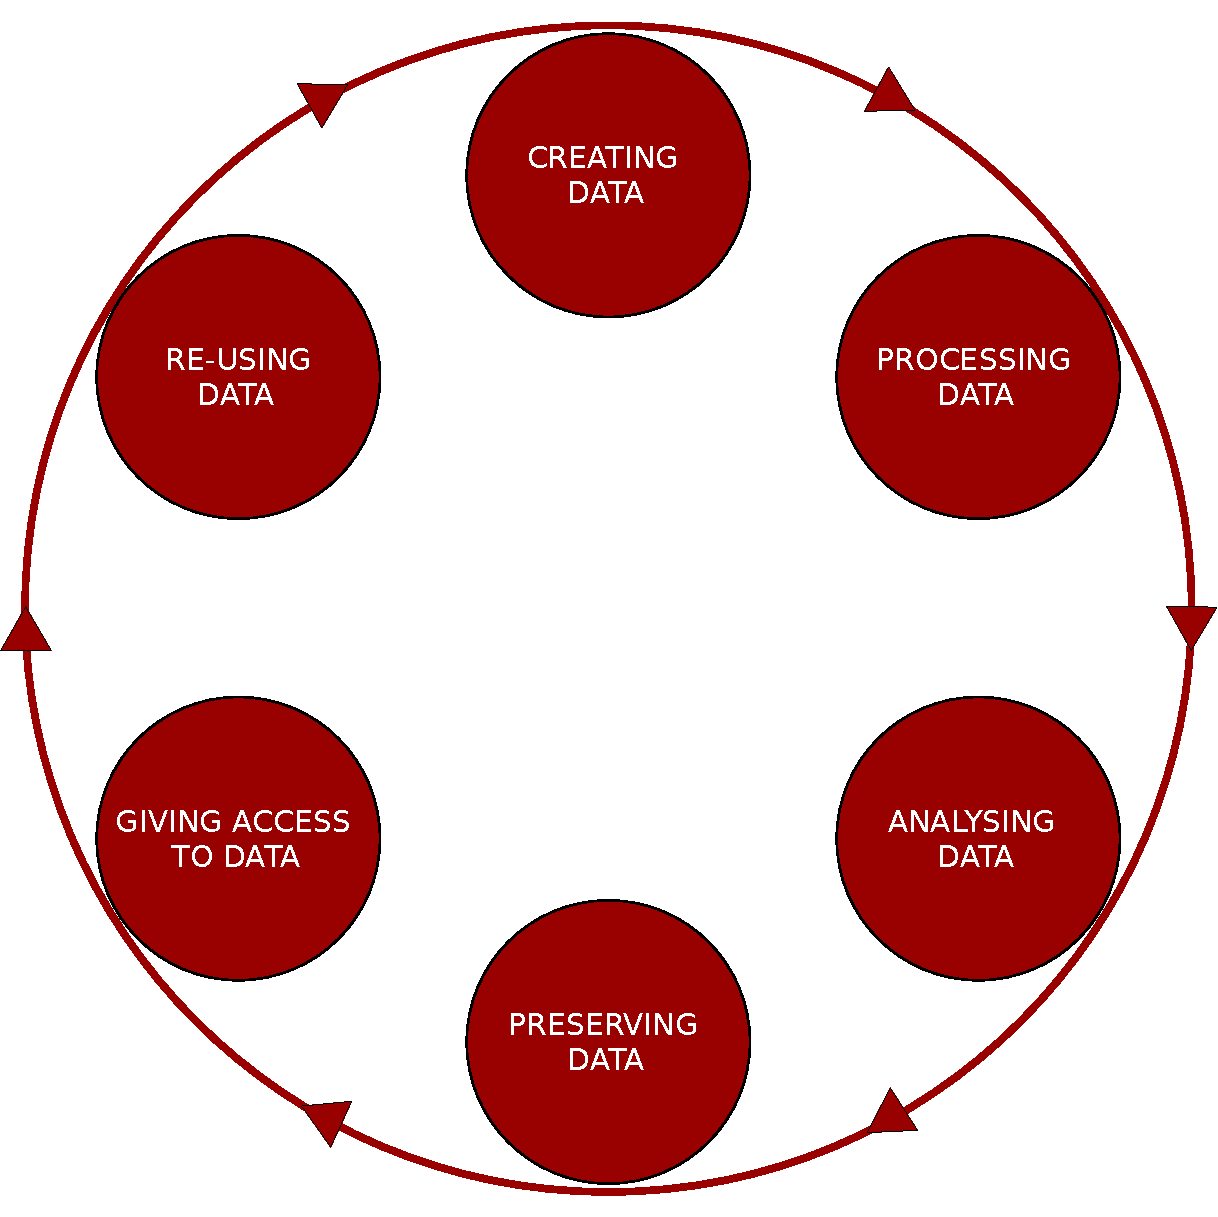
\includegraphics[height=0.7\paperheight]{graphics/research-data-lifecycle.pdf}
  \end{center}
  
  \begin{center}
     \tiny Adapted from \url{http://www.data-archive.ac.uk/create-manage/life-cycle}
  \end{center}
\end{frame}

% http://www2.le.ac.uk/services/research-data/documents/UoL_ReserchDataDefinitions_20120904.pdf
% Different from data types in programming languages (primitive, composite, abstract)
\begin{frame}
  \frametitle{Research data types}
  
  \begin{itemize}
  \item Observational data
  \begin{itemize}
    \item Result from recognizing, noting or recording facts
    \item Collected by human observation, surveys, instruments
    \item Typically difficult or impossible to reproduce
    \item Measurement of ocean temperature at locations in space-time
  \end{itemize}
  \item Experimental data
  \begin{itemize}
    \item Result of procedures in controlled conditions
    \item In theory reproducible but may be expensive
    \item Chemical analysis in a laboratory
  \end{itemize}
  \item Computational data
  \begin{itemize}
    \item Result in executing computer models, simulations, or workflows
    \item Reproducible if software and input available
    \item Plant disease pressure model
  \end{itemize}
  \end{itemize}
\end{frame}


\begin{frame}
  \frametitle{Data formats}
  
  \begin{itemize}
  \item Serialized representation of data
  \item Comma separated values (CSV) is a common format
  \item JPEG, TIFF, PNG, GIF for raster images
  \item SVG, EPS, PDF for vector graphics
  \item NetCDF, HDF5 for array scientific data
  \end{itemize}
\end{frame}

\begin{frame}
  \frametitle{Data models}
  
  \begin{itemize}
  \item Abstract formalization of objects and relationships in a domain
  \begin{itemize}
    \item There are lakes, rivers, and mountains
    \item Lakes and rivers have a depth
    \item Mountains have an elevation
    \item Rivers have a length
  \end{itemize}
  \item Set of concepts used to define formalizations
  \begin{itemize}
    \item Entity-relationship data model
    \item Graph data model
    \item Geographic data model
  \end{itemize}
  \end{itemize}
\end{frame}

\begin{frame}
  \frametitle{Standards}
  
  \begin{itemize}
  \item Heterogeneity in data models and standards hinders interoperability
  \item Characteristic of system to work with other systems
  \end{itemize}
  \begin{center}
    
\includegraphics[scale=0.5]{graphics/compatibility.png}\hspace{0.5cm}
    
\includegraphics[scale=0.47]{graphics/de-facto-standard.png}\hspace{0.5cm}
    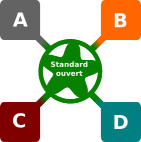
\includegraphics[scale=0.31]{graphics/interoperability.png}\\
    \tiny\url{definition-interoperabilite.info}
  \end{center}
  \begin{itemize}
  \item Syntactic and semantic interoperability
  \item If you can use (de facto) standard, recommendation, wide acceptance
  \item Examples
    \begin{itemize}
    \item ISO Date and time format, Country codes, Geographic information
    \item W3C HTML, XML, RDF
    \item IETF TCP/IP, URI
    \end{itemize}
  \end{itemize}
\end{frame}

% Descriptive metadata describes a resource for purposes such as discovery and identification. It can include elements such as title, abstract, author, and keywords.
% Structural metadata is metadata about containers of data and indicates how compound objects are put together, for example, how pages are ordered to form chapters. It describes the types, versions, relationships and other characteristics of digital materials.
% Administrative metadata provides information to help manage a resource, such as when and how it was created, file type and other technical information, and who can access it.
\begin{frame}
  \frametitle{Metadata}
  
  \begin{itemize}
  \item Metadata is data about other data
  \item Metadata describes, explains, locates data
  \item Supports discovery, retrieval, use, management of data
%  \item Descriptive, structural, administrative metadata
  \item May be created manually or automatically
  \item What is data for someone may be metadata for someone else
  \item Examples
  \begin{itemize}
    \item Data about observational data, e.g. about sensor and property
    \item Data about published data, e.g. title, authors, identifiers
    \item Phone call content vs. phone number, call duration
  \end{itemize}
  \end{itemize}
\end{frame}

\begin{frame}
  \frametitle{Data management}
  
  \begin{itemize}
  \item Organization, storage, preservation, and sharing of data 
  \item Data collected and used in a research project 
  \item Data is complicated; good management imperative
  \item From issues such as consistent file naming conventions
  \item To safeguarding access over the next 10 years
  \end{itemize}
\end{frame}

\begin{frame}
  \frametitle{Why data management}
  
  \begin{itemize}
    \item Increasingly required by funders and publishers
    \item Saves time and resources in the long run
    \item Prevents errors and increases quality of research
    \item Enables replication and validation of results
    \item Potential for new discoveries, if shared with others
  \end{itemize}
\end{frame}

\begin{frame}
  \frametitle{Planning data management}
  
  \begin{itemize}
  \item Good data management needs to be carefully planned
  \item Use planning tools, including model of data lifecycle
  \item Consider
  \begin{itemize}
    \item Data format and quantity of collected data
    \item Is data going to be versioned, tracking needed
    \item Data storage, archiving and backup policy and implementation
    \item Creating and managing metadata that describe the data
    \item Data access and sharing, license and security
    \item Budgeting data management and preservation
  \end{itemize}
  \end{itemize}
\end{frame}

% Look at DMPtool in exercise
%\begin{frame}
%  \frametitle{Tools for data management planning}
%  
%  \begin{itemize}
%  \item 
%  \end{itemize}
%\end{frame}

\begin{frame}
  \frametitle{Take aways}
  
\end{frame}

\begin{frame}
  \frametitle{References}
  \tiny
  \bibliography{../../../../../bibliography/bibliography}
  \vspace{0.5cm}
  Slide 3: Joan Mir{\'o} (1968). Landscape. Acrylic on canvas. Fundaci{\'o}n Joan Mir{\'o}, Barcelona. \url{https://www.fmirobcn.org/en/colection/catalog-works/5442/p-landscape-p}
  
  Slide 5: On defining data, see \url{http://pitt.libguides.com/managedata}
  
  Slide 14: On research data management, see \url{http://pitt.libguides.com/managedata}
\end{frame}

\end{document}
